\documentclass[11pt,a4paper]{article}
\usepackage[utf8]{inputenc}
\usepackage[T1]{fontenc}
\usepackage{lmodern}
\usepackage[english]{babel}
\usepackage{microtype}
\usepackage[a4paper,margin=2.3cm]{geometry}
\usepackage{graphicx}
\usepackage{booktabs}
\usepackage{xcolor}
\usepackage{titlesec}
\usepackage{enumitem}
\usepackage{float}
\usepackage[hidelinks]{hyperref}
\definecolor{accent}{HTML}{1F4E79}
\titleformat{\section}{\large\bfseries\color{accent}}{\thesection}{0.6em}{}
\titleformat{\subsection}{\normalsize\bfseries}{\thesubsection}{0.6em}{}
\setlist{itemsep=2pt,topsep=3pt}
\setlength{\parskip}{4pt}
\graphicspath{{../figures/}}

\begin{document}

\begin{center}
{\LARGE\bfseries\color{accent} Road accidents in France and in Haut-Rhin, 2019--2024}\\[6pt]
{\large An analysis of 309{,}756 injury accidents and 18{,}356 road deaths}\\[8pt]
Deo Gratias Loutou \,\textbar\, \href{https://github.com/LDGKM/road-accidents-france}{github.com/LDGKM/road-accidents-france} \,\textbar\, October 2026
\end{center}

\section*{Executive summary}
About \textbf{3{,}000 people die every year} on the roads of metropolitan France, and that number has not
improved since 2019: after the 2020 lockdowns, recorded accidents settled about 9\% below their 2019 level,
while deaths came back to it. The risk is concentrated in a few situations:
\begin{itemize}
  \item \textbf{Outside built-up areas}: 36\% of accidents, but \textbf{68\% of deaths}.
  \item \textbf{At night}: between 3 and 6~a.m., about 11\% of accidents are fatal, twice the daytime rate.
  \item \textbf{Young men and the elderly}: 78\% of the dead are men; death rates peak at 20--24 years and after 80.
  \item \textbf{New modes}: e-scooter deaths rose from 11 (2019) to 47 (2024), and injured e-scooter users from 677 to 2{,}746.
\end{itemize}
\textbf{Haut-Rhin} is among the safer departments, with 36 deaths per million inhabitants a year against 46
nationally (11th of 96). But the data hide a trap: Mulhouse records \emph{fewer} accidents than Colmar, a
smaller city, and 15 times fewer than Strasbourg. Minor accidents are very likely under-recorded there, so any
indicator built on accident counts (share of fatal accidents, accidents per inhabitant) is biased for this area.

\section{Question and data}
\textbf{Questions.} When, where and to whom do road deaths happen? How does Haut-Rhin compare with the rest of
France? Which circumstances turn an injury accident into a fatal one?

\textbf{Data.} The national injury-accident file (BAAC) published by the road-safety observatory ONISR on
data.gouv.fr: one record for every accident with at least one injured person reported by the police or
gendarmerie, in four tables per year (accidents, places, vehicles, people). We use 2019--2024, the years
with a stable format, and metropolitan France only (96 departments). Population figures come from
INSEE's estimates on 1~January 2023, by department, sex and five-year age group.

\begin{table}[H]\centering\small
\begin{tabular}{lrlp{6.2cm}}\toprule
Table & Rows (2019--2024) & Grain & Main fields used \\\midrule
Accidents & 327{,}628 & one accident & date, hour, light, department, commune, built-up area, weather, collision type, GPS \\
Places & 327{,}628 & one accident & road category, speed limit, surface \\
Vehicles & 559{,}847 & one vehicle & vehicle category, obstacle hit \\
People & 745{,}158 & one person & role, injury severity, sex, year of birth \\\bottomrule
\end{tabular}
\caption{Raw tables (France incl.\ overseas). Metropolitan scope: 309{,}756 accidents.}
\end{table}

\section{Method}
\textbf{Cleaning (SQL, DuckDB).} The 24 CSV files are loaded as text and typed in SQL
(file \texttt{sql/01\_clean.sql}). The open data change format between years: the 2022 accident id column is named
\texttt{Accident\_\allowbreak Id}, missing values appear as \texttt{" -1"}, \texttt{"(1)"} or \texttt{"N/A"}, coordinates use
decimal commas, some years write department \texttt{"1"} instead of \texttt{"01"}. A single SQL macro turns every
coded field into an integer or NULL; speed limits outside 10--130~km/h (e.g.\ 500, 900) are set to NULL.

\textbf{Modelling the data.} Vehicle categories (about 40 official codes) are grouped into 11 travel modes;
pedestrians, who are attached to the vehicle that hit them, get their own mode. A view gives one row per
accident with its outcome (deaths within 30 days, injuries) and its risk factors (\texttt{sql/02\_model.sql}).

\textbf{Validation.} Data quality is high: less than 2.3\% missing on every field used. Our death counts match
the official ONISR figures \emph{exactly} for 2019 to 2023 (3{,}244; 2{,}541; 2{,}944; 3{,}267; 3{,}167), which
shows that cleaning and filtering lose no accident. We do not use the ``hospitalised'' category on its own:
since 2019 it is no longer certified by the public statistics authority.

\textbf{Statistics.} Rates per inhabitant use INSEE 2023 population (also for 2024, not yet published at
department level). The fatality model is a logistic regression (statsmodels) on 301{,}290 accidents with
complete fields, with year fixed effects; it is checked out of sample on a 25\% hold-out.

\section{Findings}
\subsection{A plateau since 2019}
\begin{figure}[H]\centering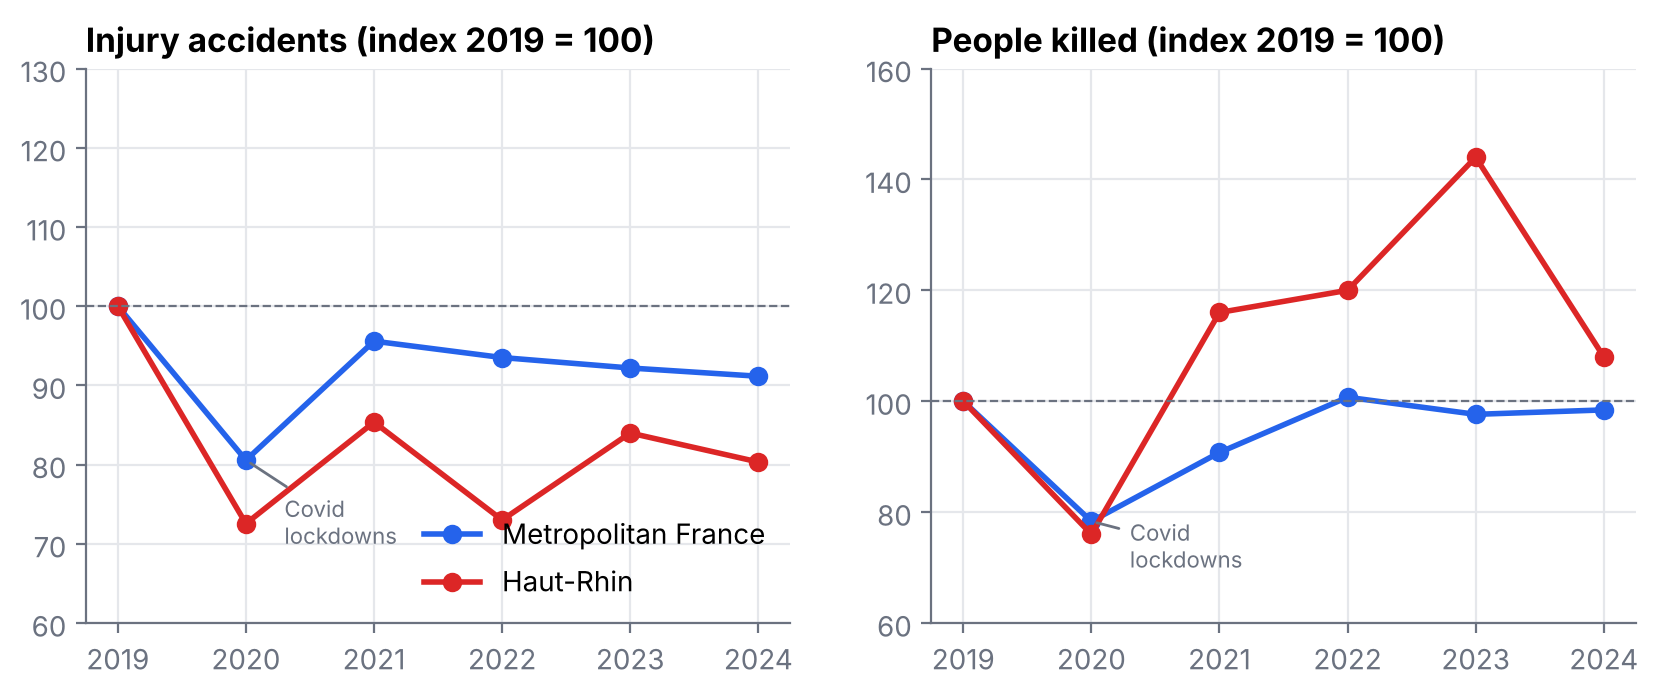
\includegraphics[width=\linewidth]{01_trend}\end{figure}
Both series dropped in 2020. Deaths returned to their 2019 level from 2022 (3{,}193 in 2024) while recorded
accidents stayed about 9\% lower. Haut-Rhin follows the same path, but with 19 to 36 deaths a year its
yearly swings are mostly random and should not be over-interpreted.

\subsection{When: rush hour for accidents, small hours for deaths}
\begin{figure}[H]\centering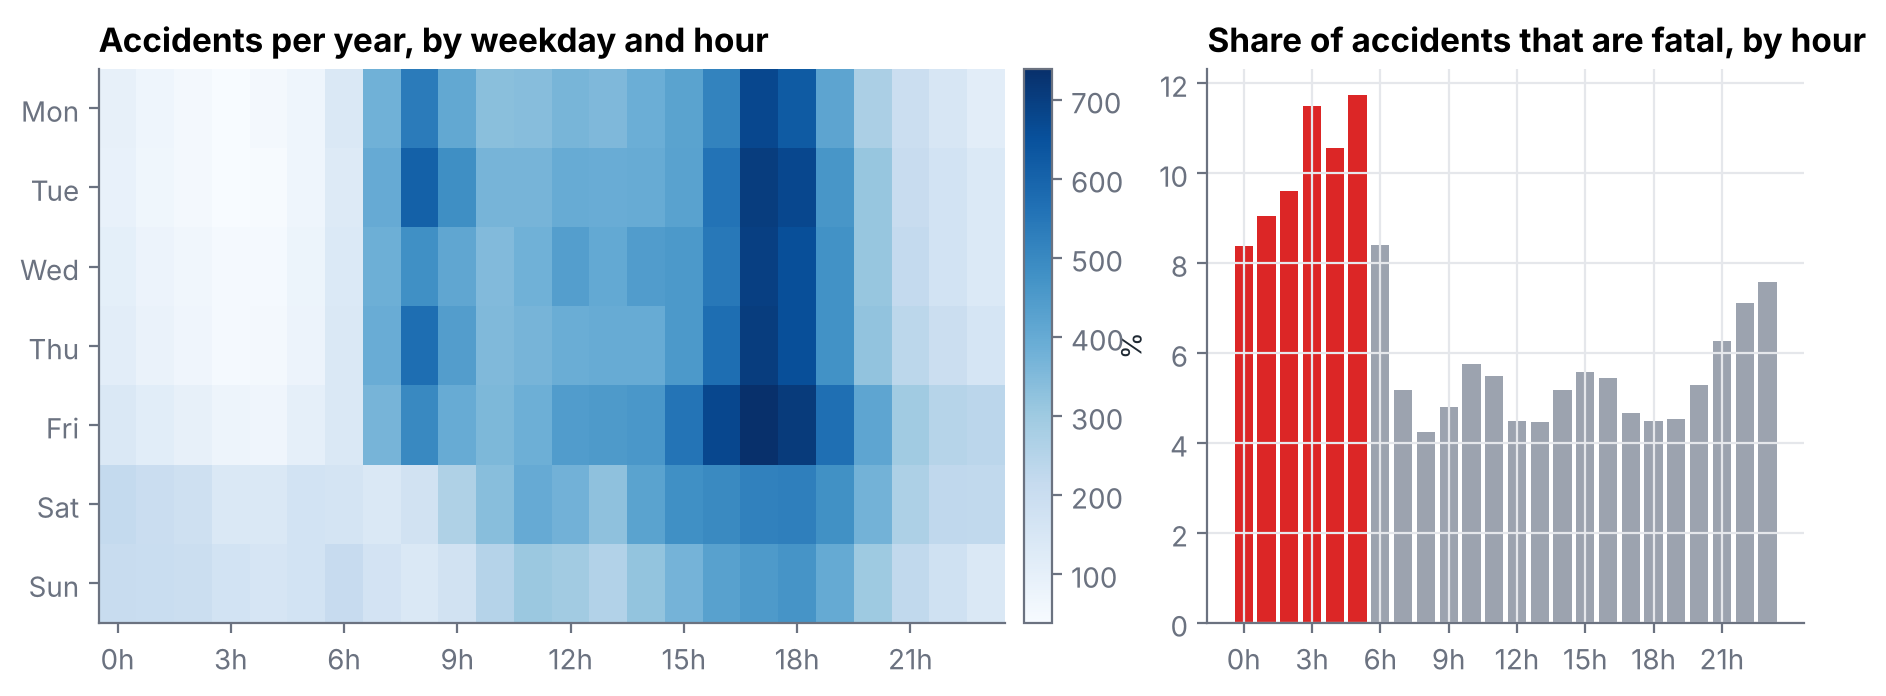
\includegraphics[width=\linewidth]{02_when}\end{figure}
The busiest slot is Friday 5--6~p.m. But accidents in the small hours are far more severe: 11\% are fatal
between 3 and 6~a.m.\ against 4.5--5.5\% during the day (higher speeds, fatigue, alcohol and fewer witnesses
are the usual explanations; the data cannot separate them). Night accidents represent 26\% of accidents and
35\% of deaths.

\subsection{Who: car occupants first, but e-scooters are rising fastest}
\begin{figure}[H]\centering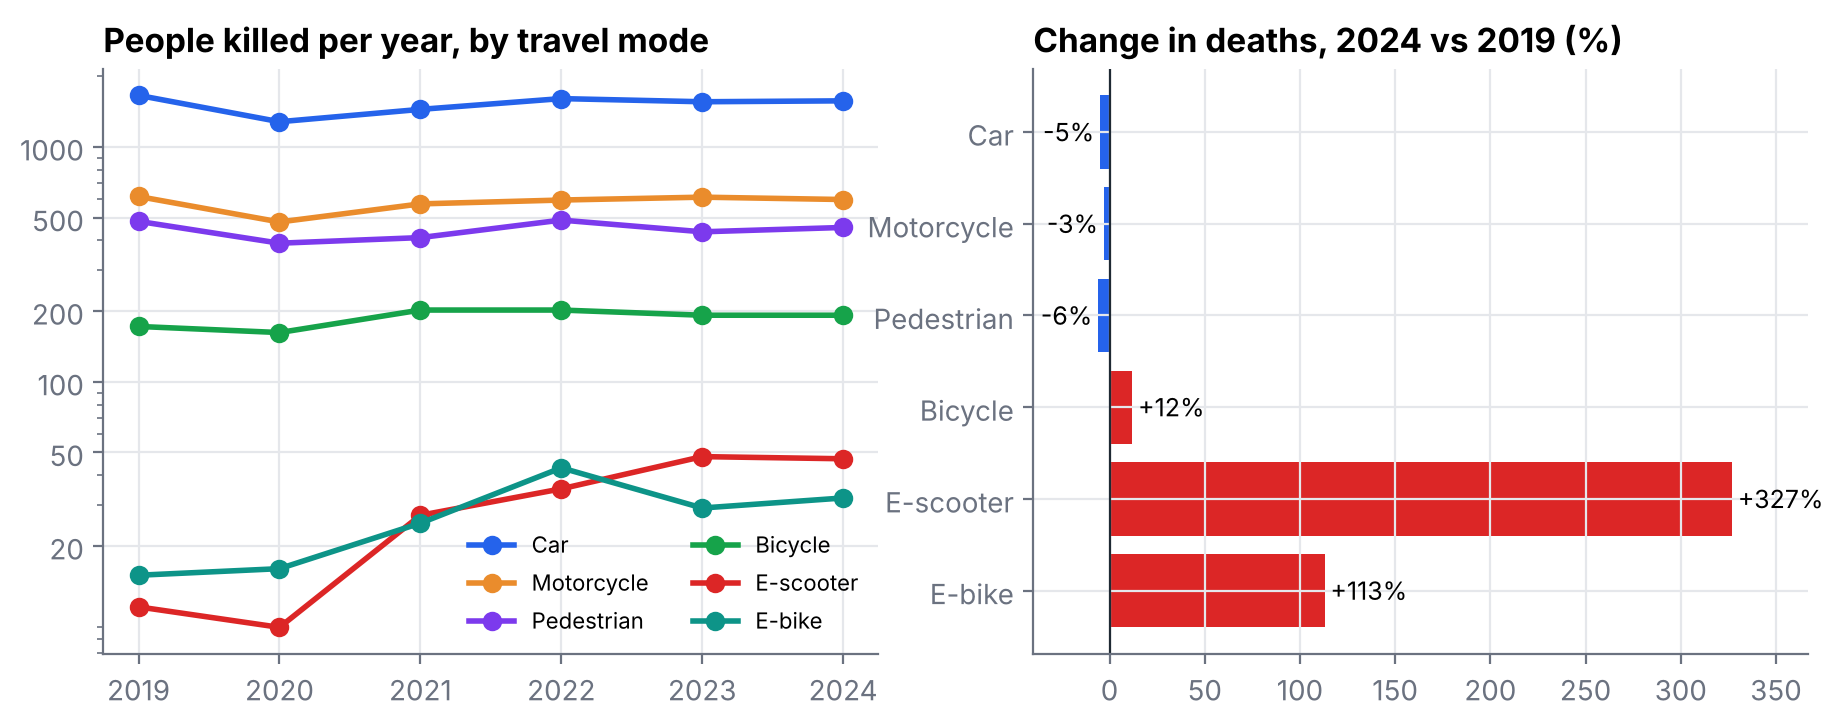
\includegraphics[width=\linewidth]{03_modes}\end{figure}
Car occupants (about 1{,}600 deaths a year), motorcyclists (600) and pedestrians (450--480) dominate.
Their numbers barely moved between 2019 and 2024. The change comes from new modes: deaths on e-scooters
went from 11 to 47 and on e-bikes from 15 to 32, while the number of injured e-scooter users quadrupled.
\begin{figure}[H]\centering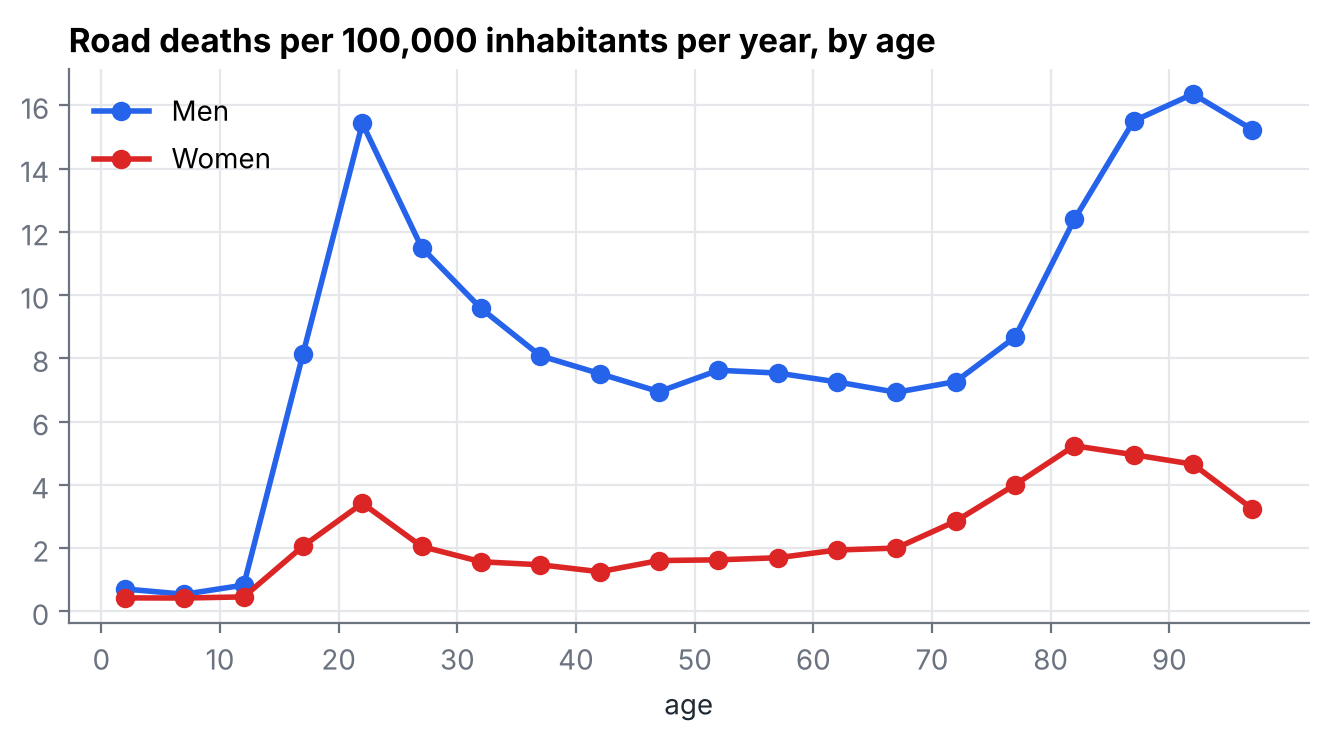
\includegraphics[width=0.8\linewidth]{04_age}\end{figure}
Men account for 78\% of deaths. For men, the death rate jumps to 15 per 100{,}000 at 20--24, twice
the rate at 40--60, and climbs back after 80 (frailty: the same crash is deadlier at that age).

\subsection{Where: rural roads kill}
Accidents outside built-up areas are a third of the total but two thirds of the deaths. The map shows the
consequence: the most urban departments (Paris and its inner suburbs, Rhône) have the lowest death rates per
inhabitant, the rural centre and south the highest (up to 97 per million).
\begin{figure}[H]\centering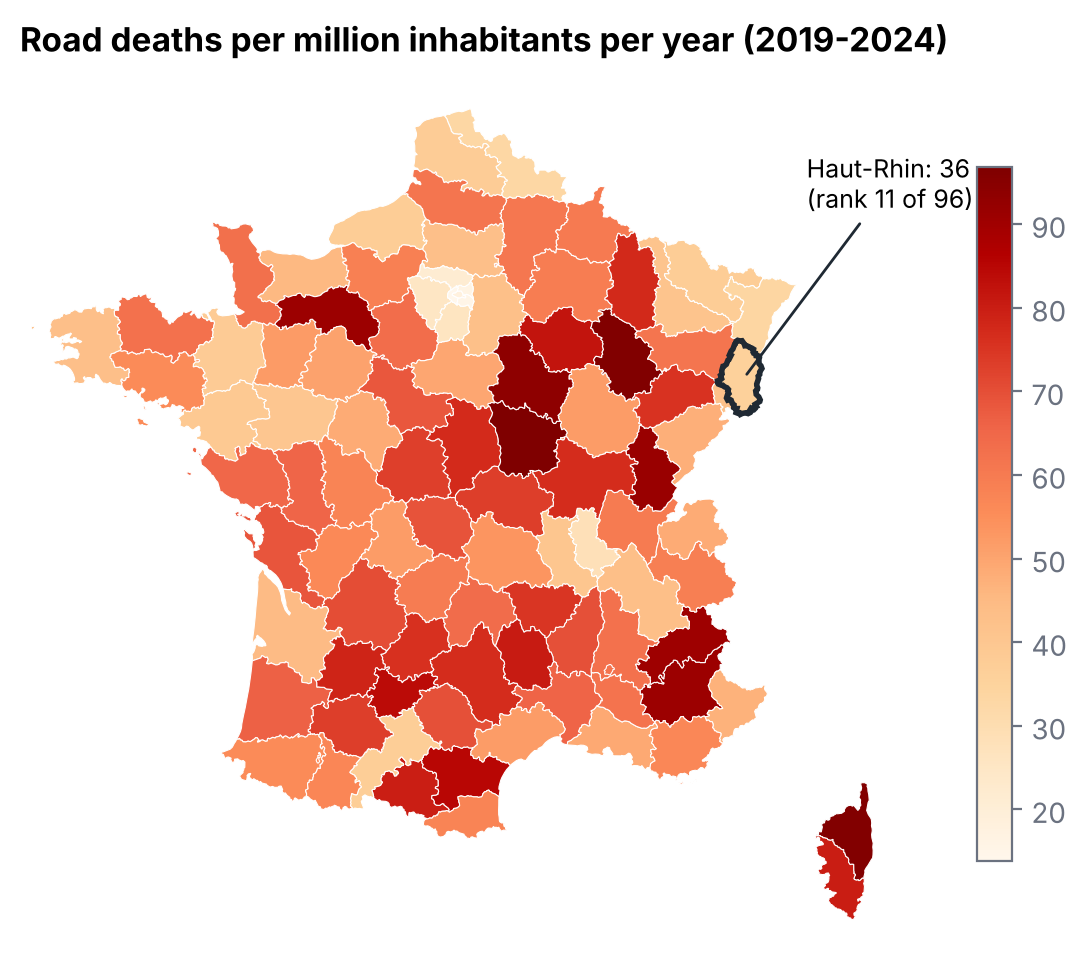
\includegraphics[width=0.72\linewidth]{05_map_departments}\end{figure}

\subsection{Haut-Rhin}
With 36 deaths per million inhabitants a year, Haut-Rhin ranks 11th safest of 96 departments, well below the
national 46. Compared with the other departments, its recorded accidents happen less often in towns (53\% vs
64\%), involve more bicycles and e-scooters (17\% vs 14\%), and are more often fatal (7.2\% vs 5.6\%).
\begin{figure}[H]\centering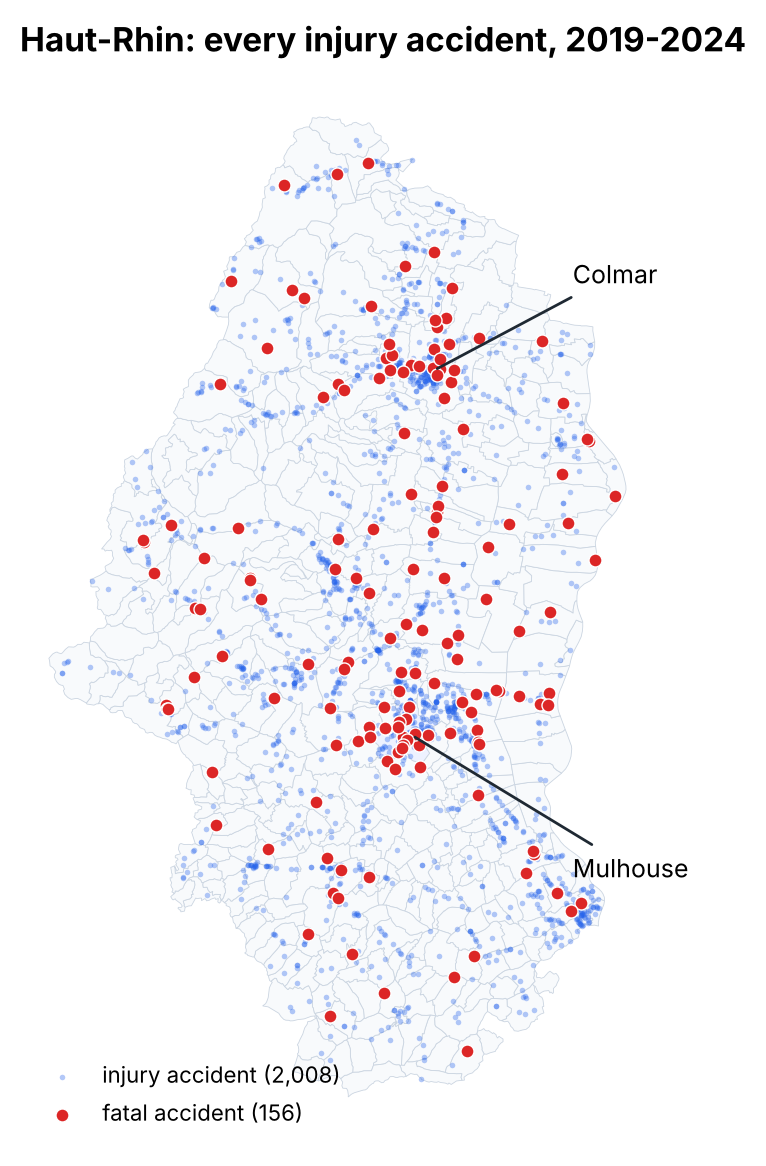
\includegraphics[width=0.6\linewidth]{06_haut_rhin_map}\end{figure}

\textbf{A recording bias.} That last figure is a warning sign rather than a finding. Deaths are almost never
missed by the police, minor injury accidents often are. Haut-Rhin records 469 accidents per million
inhabitants a year, against 785 nationally. The city level makes it obvious:
\begin{table}[H]\centering\small
\begin{tabular}{lrrr}\toprule
 & Strasbourg & Colmar & Mulhouse \\\midrule
Recorded accidents per year (2019--2024 average) & 266 & 28 & 17 \\
Deaths, 2019--2024 & 30 & 13 & 13 \\\bottomrule
\end{tabular}
\end{table}
Mulhouse, with about 105{,}000 inhabitants, records fewer accidents than Colmar (about 68{,}000) and 15 times
fewer than Strasbourg, which is only about three times larger, while it has as many deaths as Colmar. The most
likely explanation is that many non-fatal accidents in Mulhouse are not entered in the national file (they are
recorded by different police services, or not at all). Consequence for the analysis: for this area, only
indicators based on deaths are reliable. \emph{To check:} the accident records of the city of Mulhouse or of
the local police.
\begin{figure}[H]\centering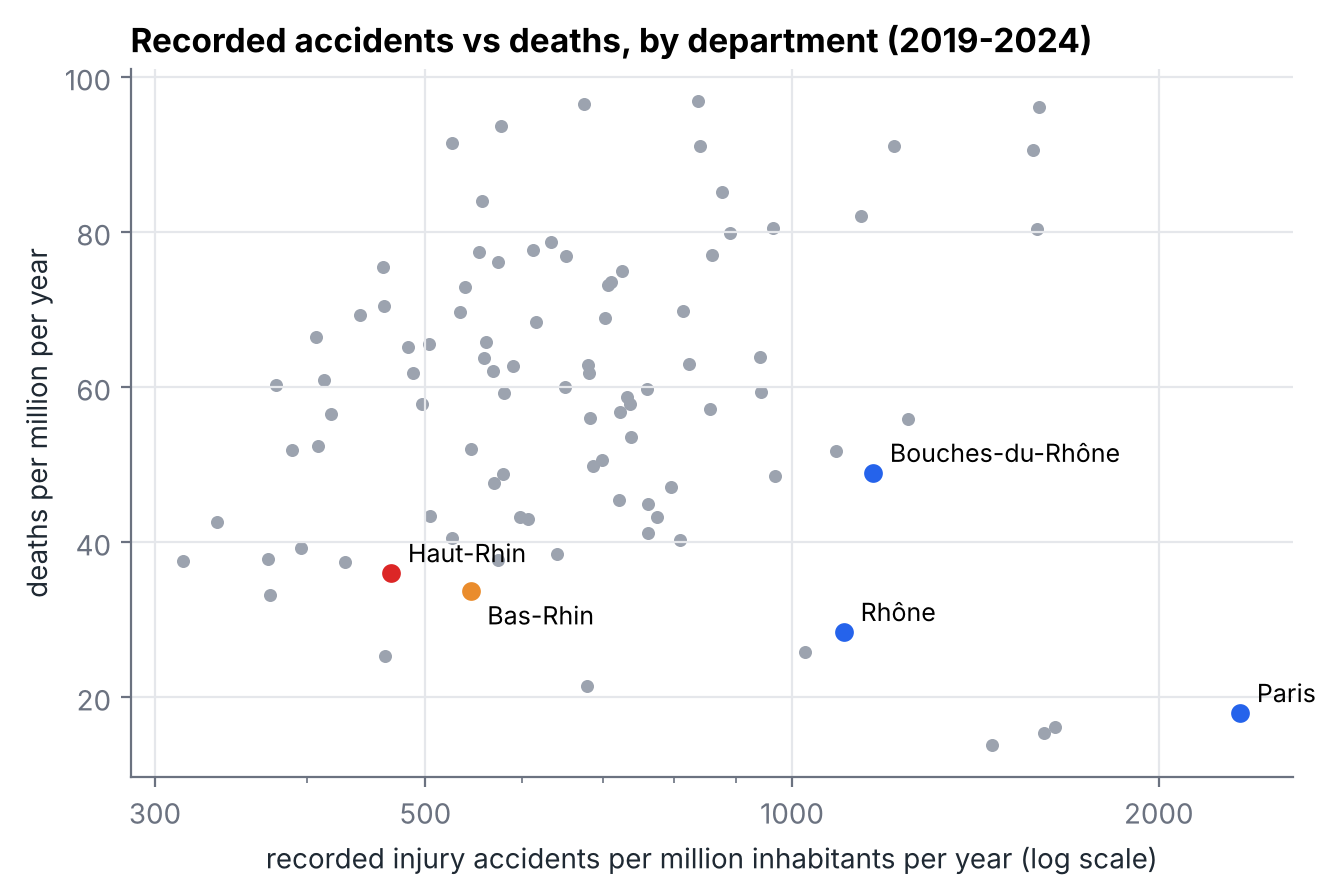
\includegraphics[width=0.75\linewidth]{07_recording_completeness}\end{figure}

\subsection{What turns an accident into a fatal one}
\begin{figure}[H]\centering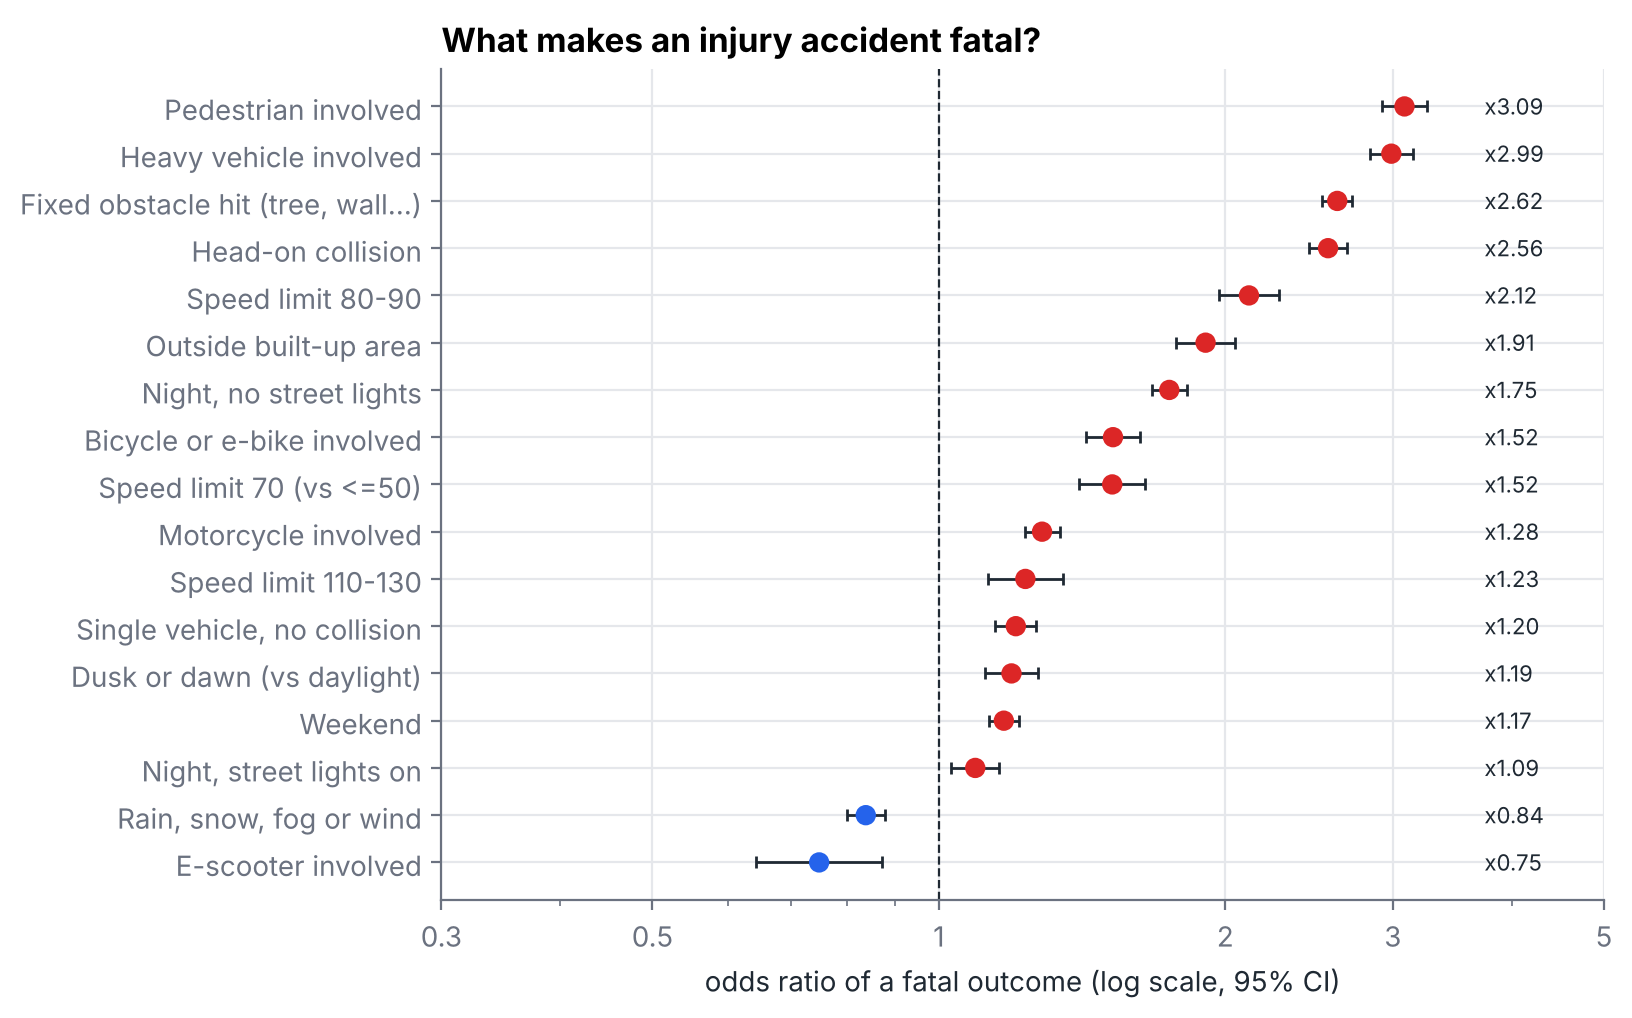
\includegraphics[width=0.85\linewidth]{08_odds_ratios}\end{figure}
Holding the other factors constant, the odds that an injury accident is fatal are multiplied by about 3 when a
pedestrian or a heavy vehicle is involved, by 2.6 when a fixed obstacle (tree, wall) is hit or in a head-on
collision, by 2.1 on 80--90~km/h roads compared with 50~km/h zones, and by 1.75 at night without street lights.
Two results look counter-intuitive and illustrate why these are associations, not causes: bad weather
\emph{lowers} the odds (0.84; drivers slow down, and rain adds many minor accidents), and so do e-scooters
(0.75; most e-scooter accidents are low-speed urban falls, even if the number of deaths is rising).
The model ranks accidents reasonably well (ROC AUC 0.76 on unseen data) but explains only part of the
outcome (pseudo-$R^2$ 0.11): speed at impact, alcohol and seat-belt use are not in the open data.

\section{Limitations}
\begin{itemize}
  \item \textbf{Police-recorded data only}: accidents without police involvement are missing, unevenly across
        places (see Mulhouse). Deaths are the most reliable indicator.
  \item \textbf{No exposure data}: we do not know kilometres travelled by mode or by road, so ``e-scooter deaths
        rose'' may partly reflect more e-scooter trips.
  \item \textbf{Population of 2023} used for all years; differences are negligible at this scale.
  \item \textbf{Small numbers} in Haut-Rhin: yearly figures fluctuate randomly.
\end{itemize}

\section{Recommendations and next steps}
\begin{enumerate}
  \item Target rural roads at night: they concentrate the deaths, not the accidents.
  \item Follow e-scooters and e-bikes closely: the fastest-growing group of victims, with exposure data
        (rental operators' trip counts) to compute real risk rates.
  \item For Mulhouse, reconcile the national file with local records before using accident counts.
  \item Extend the model with 2005--2018 data (older format) and test a gradient-boosting model for prediction.
\end{enumerate}

\section*{Reproducibility}
Code, SQL and notebook: \href{https://github.com/LDGKM/road-accidents-france}{github.com/LDGKM/road-accidents-france}.
\texttt{python run\_all.py} downloads the data and regenerates every table and figure in about two minutes.
Tools: Python, DuckDB (SQL), pandas, statsmodels, scikit-learn, matplotlib.
Data: ONISR (BAAC, Licence Ouverte 2.0), INSEE population estimates.

\end{document}
